\PassOptionsToPackage{unicode}{hyperref}
\documentclass[aspectratio=1610, 9pt]{beamer}

% Load packages you need here
\usepackage{polyglossia}
\setmainlanguage{german}

\usepackage{csquotes}
\usepackage{graphicx}
\usepackage{siunitx}
\usepackage{amsmath}
\usepackage{amssymb}
\usepackage{mathtools}

\usepackage{hyperref}
\usepackage{bookmark}

% load the theme after all packages

\usetheme[
  %showtotalframes, % show total number of frames in the footline
   % dark, % optional dark theme, uncomment to use
]{tudo}

% Put settings here, like
\unimathsetup{
  math-style=ISO,
  bold-style=ISO,
  nabla=upright,
  partial=upright,
  mathrm=sym,
}
\begin{document}
\title{Observing the Prompt Component of the Atmospheric Muon Flux Using IceCube}
\date{3 April 2025}
\author{Leander Flottau}
%\institute{Astroteilchenphysik \\  Fakultät: Physik}
\titlegraphic{
\includegraphics[width=0.7\textwidth]{Plots/IceCube_webheader_fullcolor}}
\begin{document}
\maketitle
%\begin{frame}
%  \frametitle{Table of Contents}
%  \tableofcontents
%\end{frame}  
%\section{IceCube Neutrino Observatory}
\begin{frame}
    \frametitle{IceCube Neutrino Observatory}
    \begin{minipage}{0.6\textwidth}
        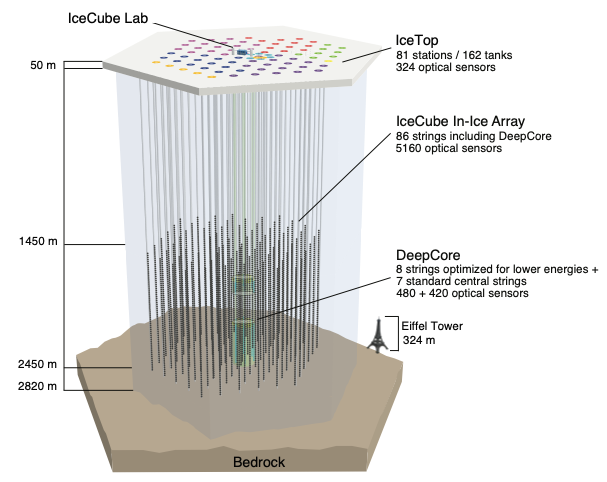
\includegraphics[width=\textwidth]{Plots/IceCube schematic}
    \end{minipage}
    \begin{minipage}{0.39\textwidth}
        \begin{itemize}
            \item Cubic kilometer scale cherenkov detector
            \item $5160$ DOMs on $86$ strings
            %\item ~$270$ measured neutrino Events per day
            \item ~$\approx \SI{3}{\kilo\hertz}$ muon event rate
        \end{itemize}
    \end{minipage}
\end{frame}
\begin{frame}
    \frametitle{Atmospheric Air Showers}
%    \begin{minipage}{0.6\textwidth}
    \begin{figure}
        \centering
        \includegraphics[width=0.6\textwidth]{Plots/Air Shower Illustration}
    \end{figure}
%    \end{minipage}
%    \begin{minipage}{0.39\textwidth}
%        \begin{itemize}
%            \item Cosmic ray interactions produce secondary particles
%            \item Major decay product: $\mu$
%        \end{itemize}
%    \end{minipage}
\end{frame}
\begin{frame}
    \frametitle{The Prompt Component}
    \begin{minipage}{0.6\textwidth}
        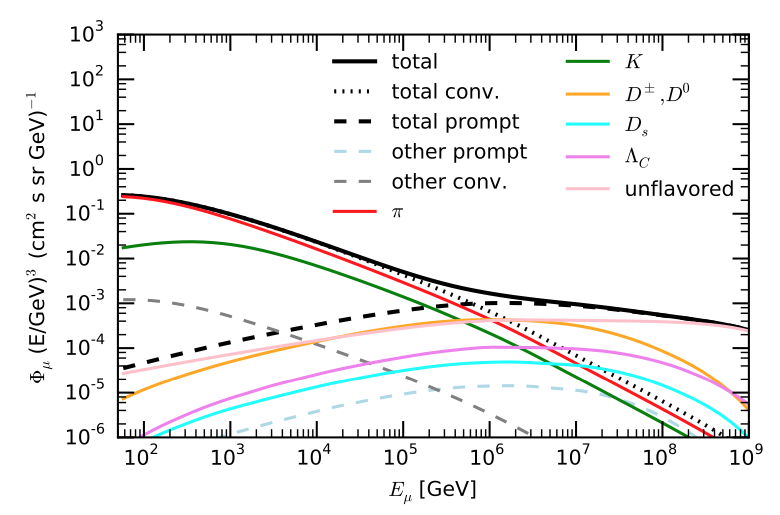
\includegraphics[width=\textwidth]{Plots/Prompt vs conventional flux}
    \end{minipage}
    \begin{minipage}{0.39\textwidth}
        \begin{itemize}
            \item Conventional: produced by $K^{\pm}$/$\pi^{\pm}$
            \item Prompt: produced by short lived particles
            \item Prompt dominant at high energies
        \end{itemize}
    \end{minipage}
\end{frame}
\begin{frame}
    \frametitle{Prompt sensitivity}
    \begin{figure}
        \centering
        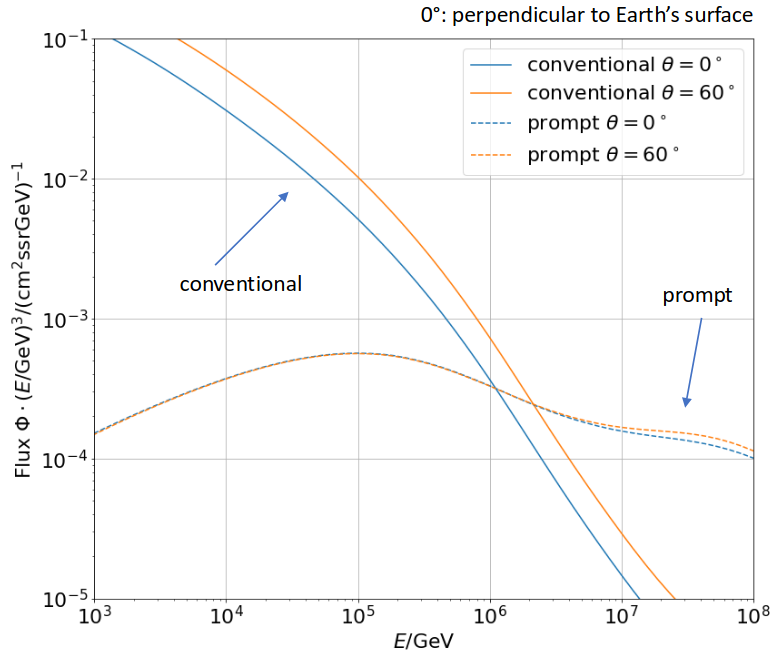
\includegraphics[width=0.8\textwidth]{Plots/prompt_flux_zenith}
    \end{figure}
\end{frame}
\begin{frame}
    \frametitle{The Muon-Puzzle}
    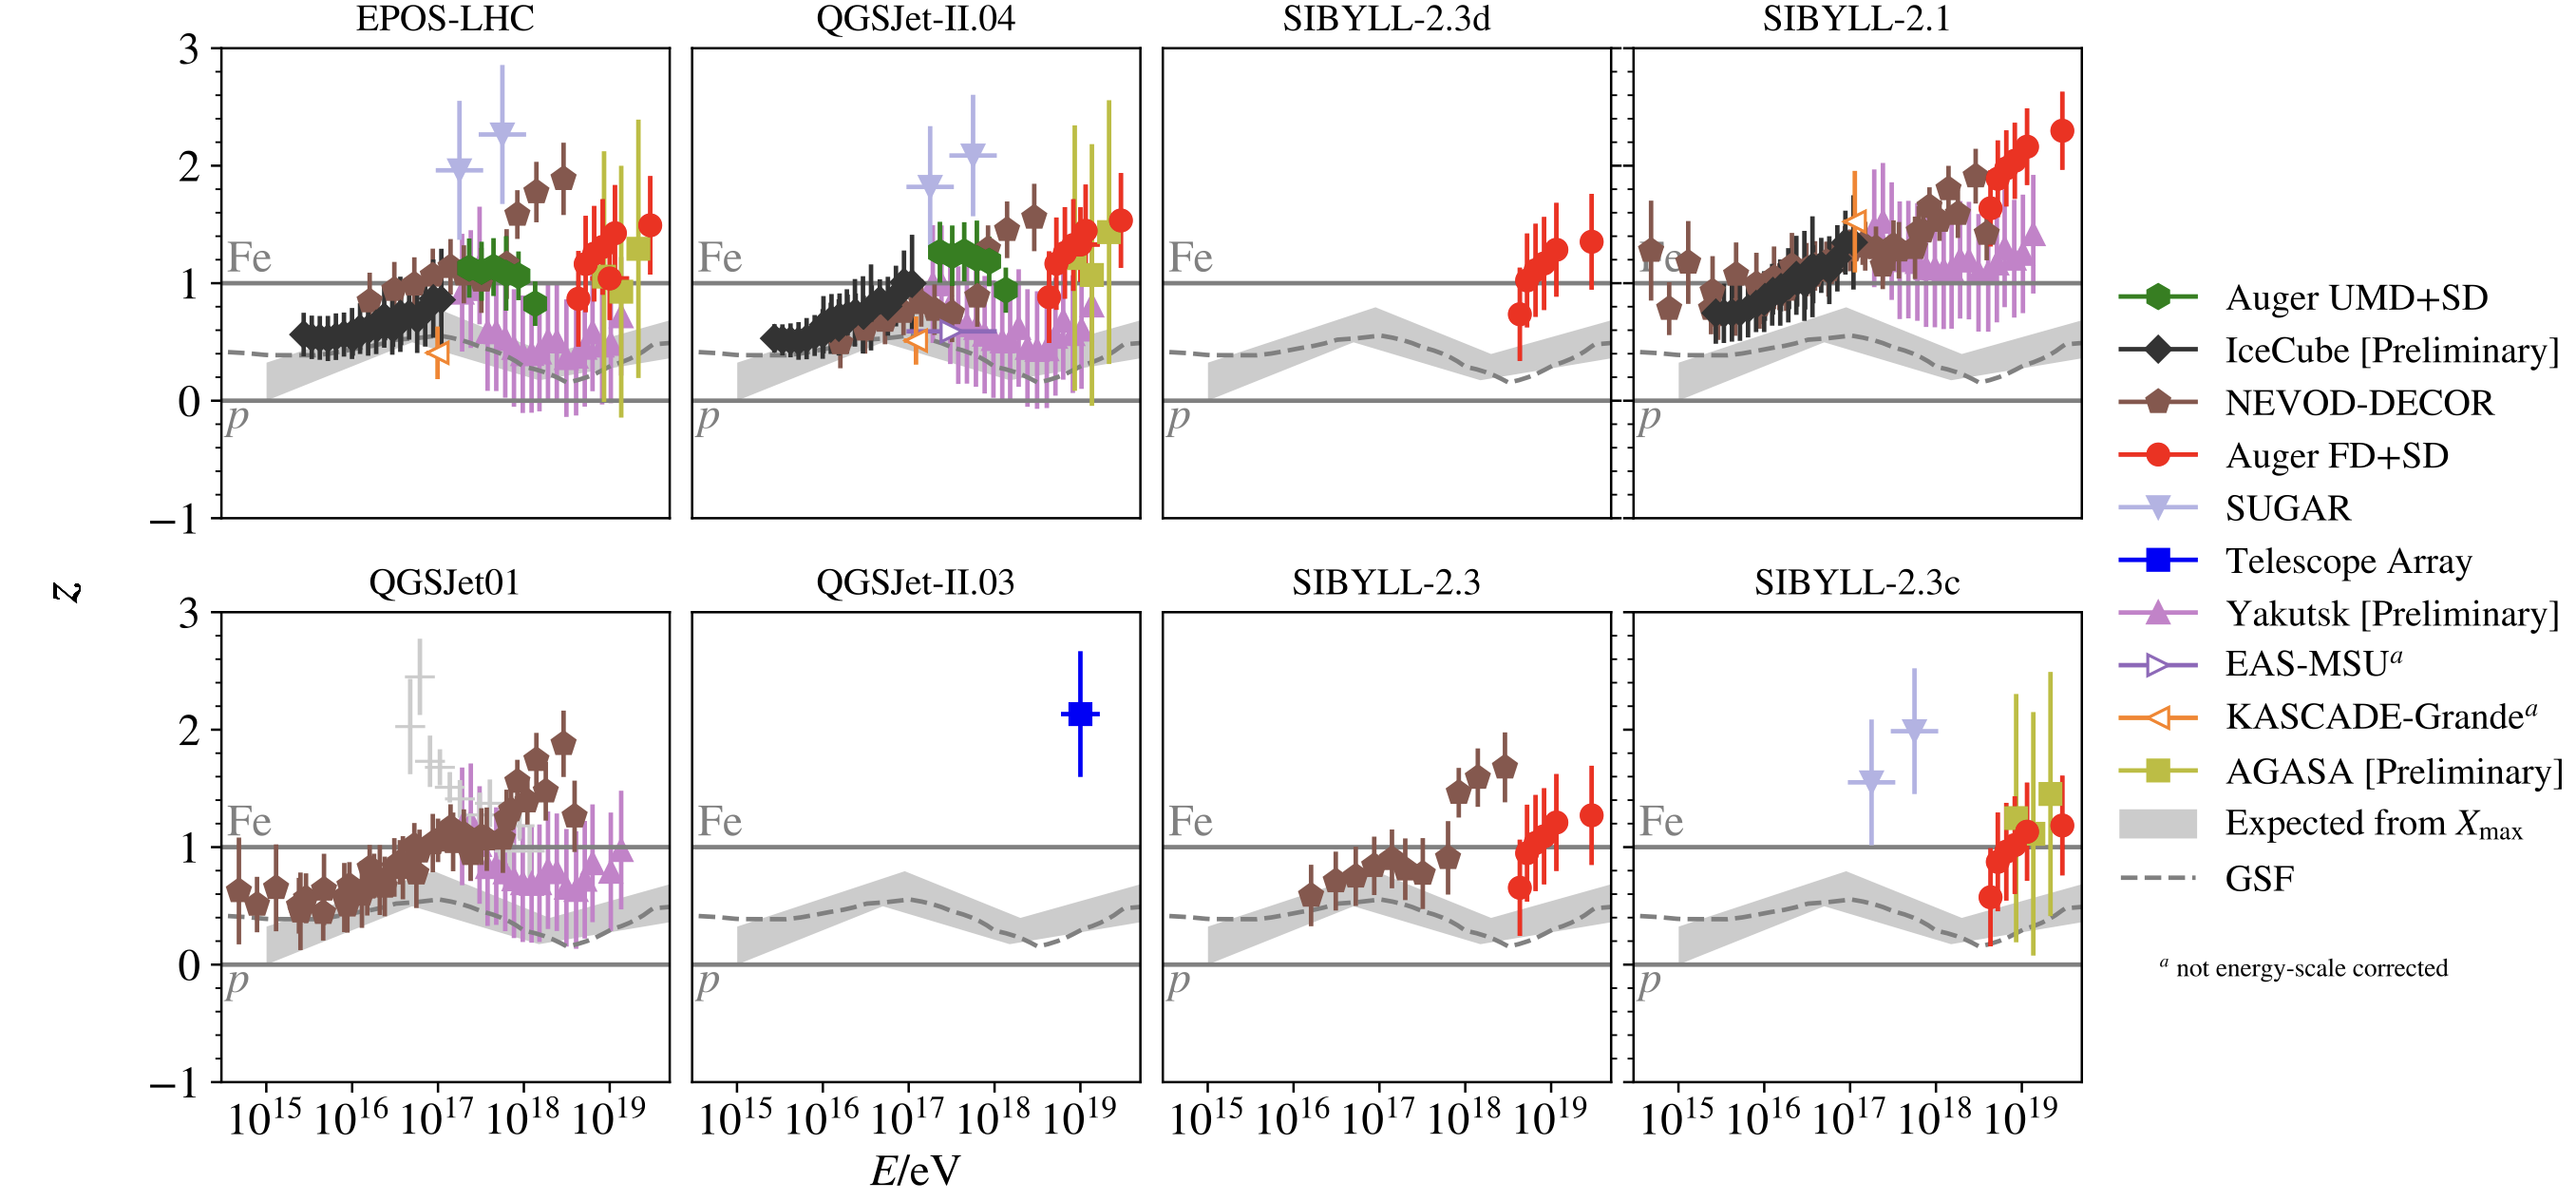
\includegraphics[width=0.9\textwidth]{Plots/muon puzzle}
%    \begin{itemize}
%        \item More muons measured than simulations predicted
%        \item Hadronic interaction models
%    \end{itemize}
\end{frame}
\begin{frame}
    \frametitle{Simulations and tagging}
    \begin{minipage}{0.5\textwidth}
        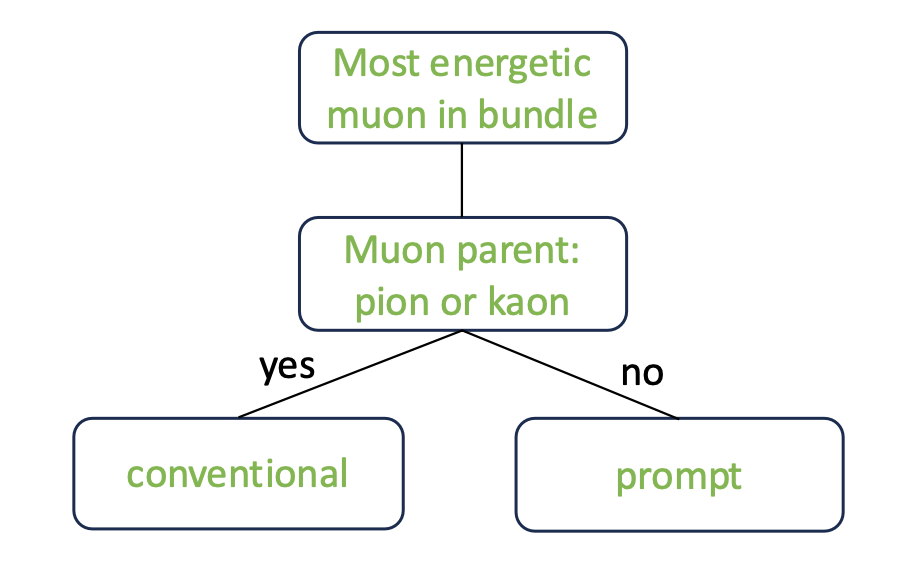
\includegraphics[width=0.8\textwidth]{Plots/prompt_tagging}
    \end{minipage}
    \begin{minipage}{0.49\textwidth}
        \begin{itemize}
            \item Tagging of parent particles in CORSIKA simulations
            \item Prompt definition based on parent of leading muon
%        \item Allows for MC-Sample with prompt/conventional distinction 
            \item Simulation up to extremely high energies
        \end{itemize}
    \end{minipage}
\end{frame}
\begin{frame}
    \frametitle{Reconstructions}
    \begin{minipage}{0.6\textwidth}
        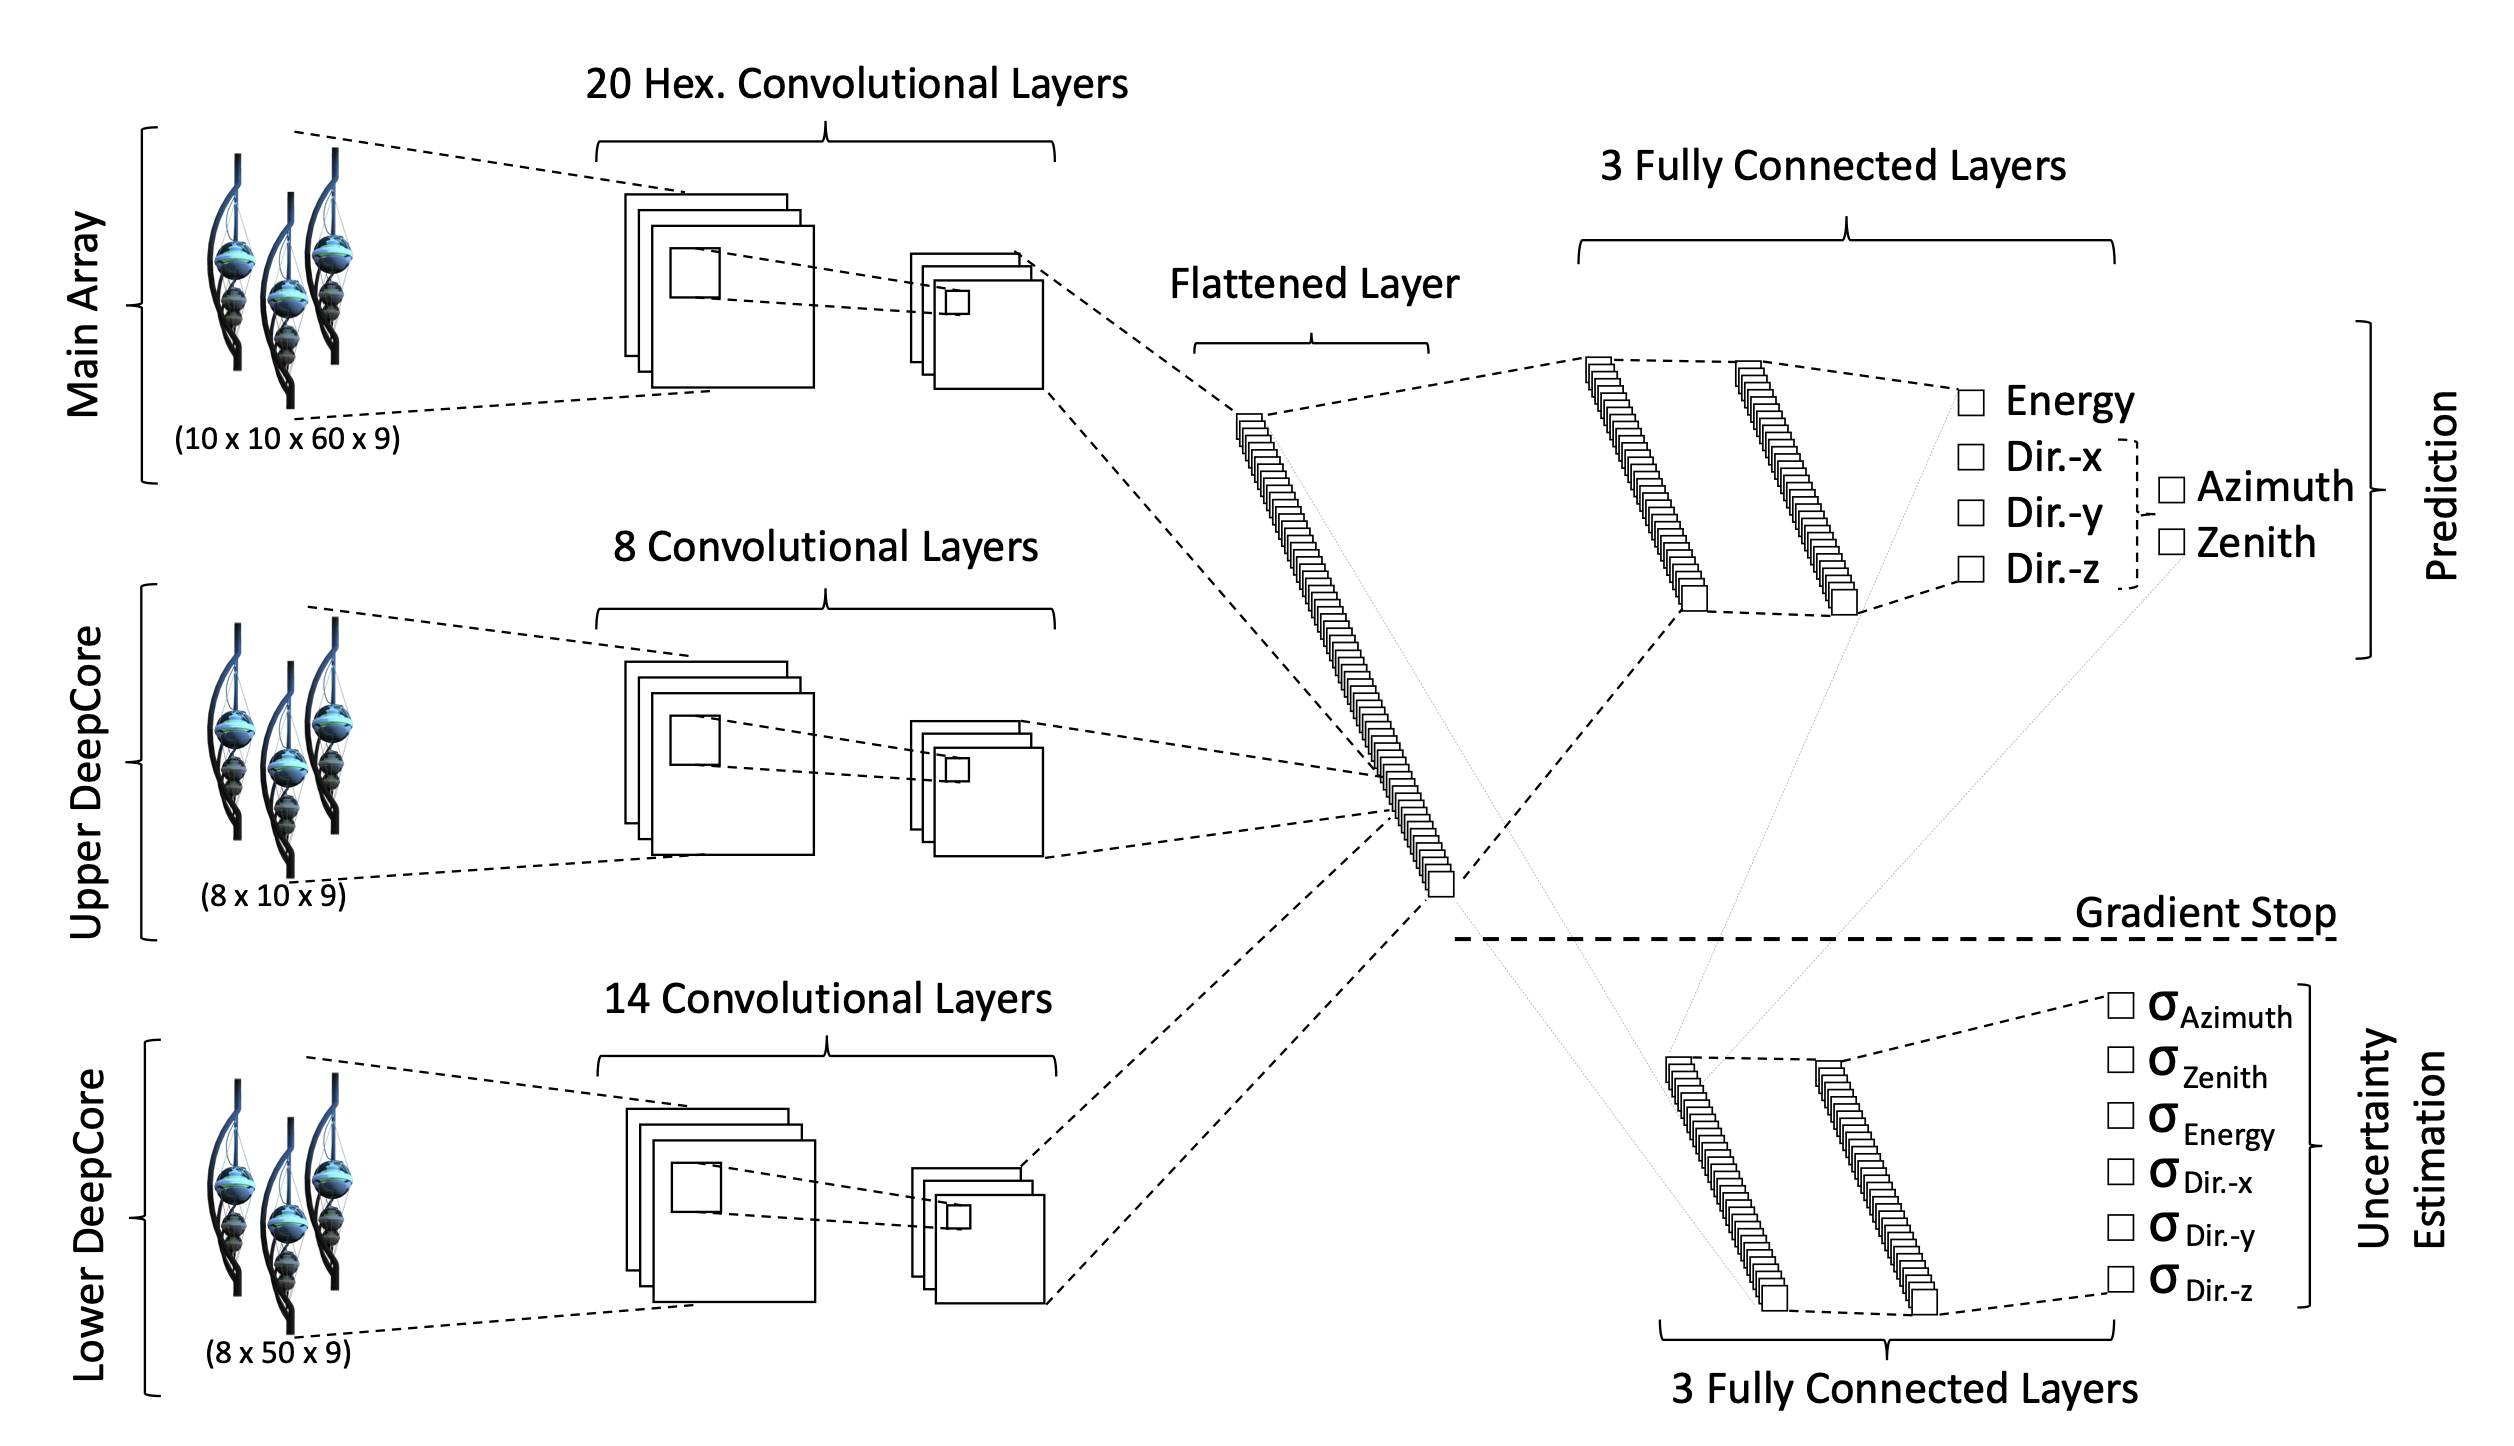
\includegraphics[width=\textwidth]{Plots/DNN_architecture}
    \end{minipage}
    \begin{minipage}{0.39\textwidth}
        \begin{itemize}
            \item Neural network based
            \item Zenith angle, bundle energy and leading muon energy
        \end{itemize}
    \end{minipage}
\end{frame}
\begin{frame}
	\frametitle{Reconstructions}
    \begin{figure}
        \centering
        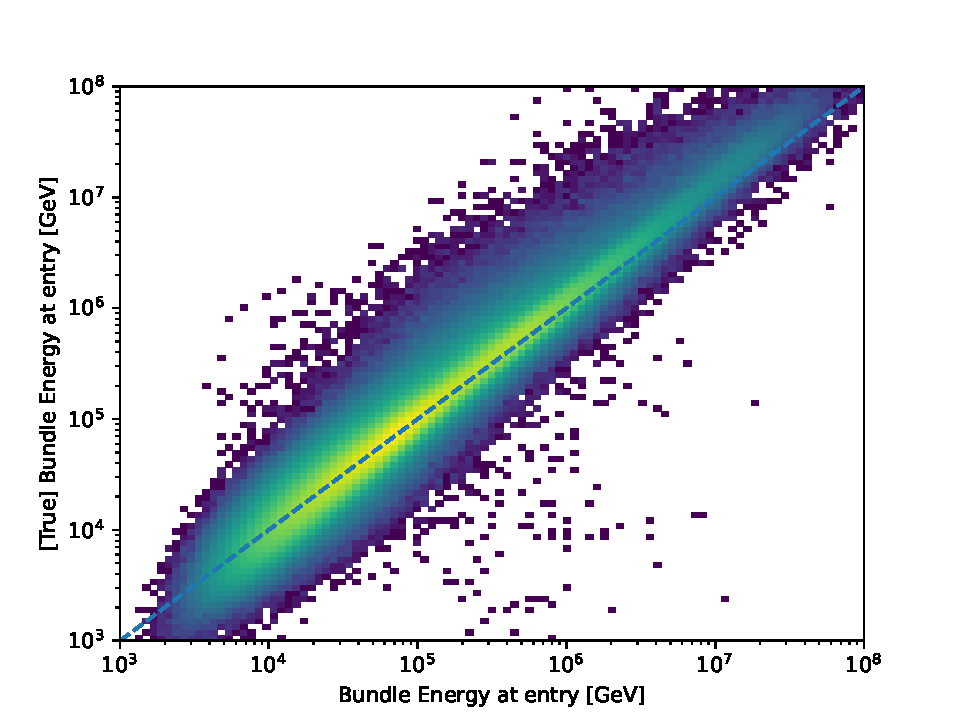
\includegraphics[width=0.49\textwidth]{Plots/bundle_correlation.pdf}
        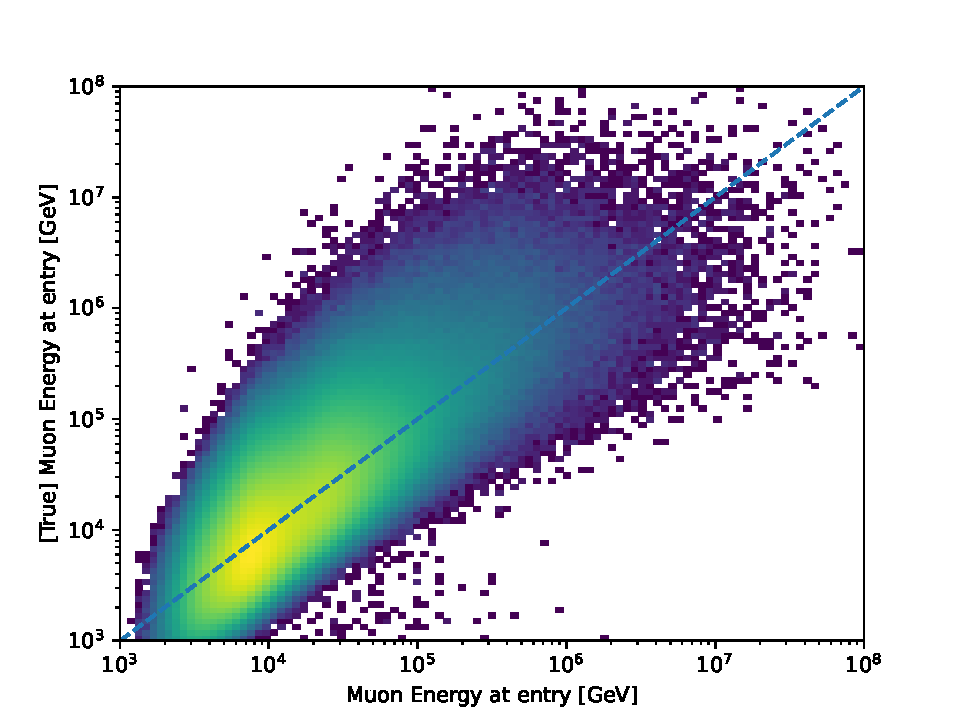
\includegraphics[width=0.49\textwidth]{Plots/entry_correlation.pdf}
    \end{figure}
\end{frame}
\begin{frame}
    \frametitle{Forward Folding}
    \begin{minipage}{0.6\textwidth}
        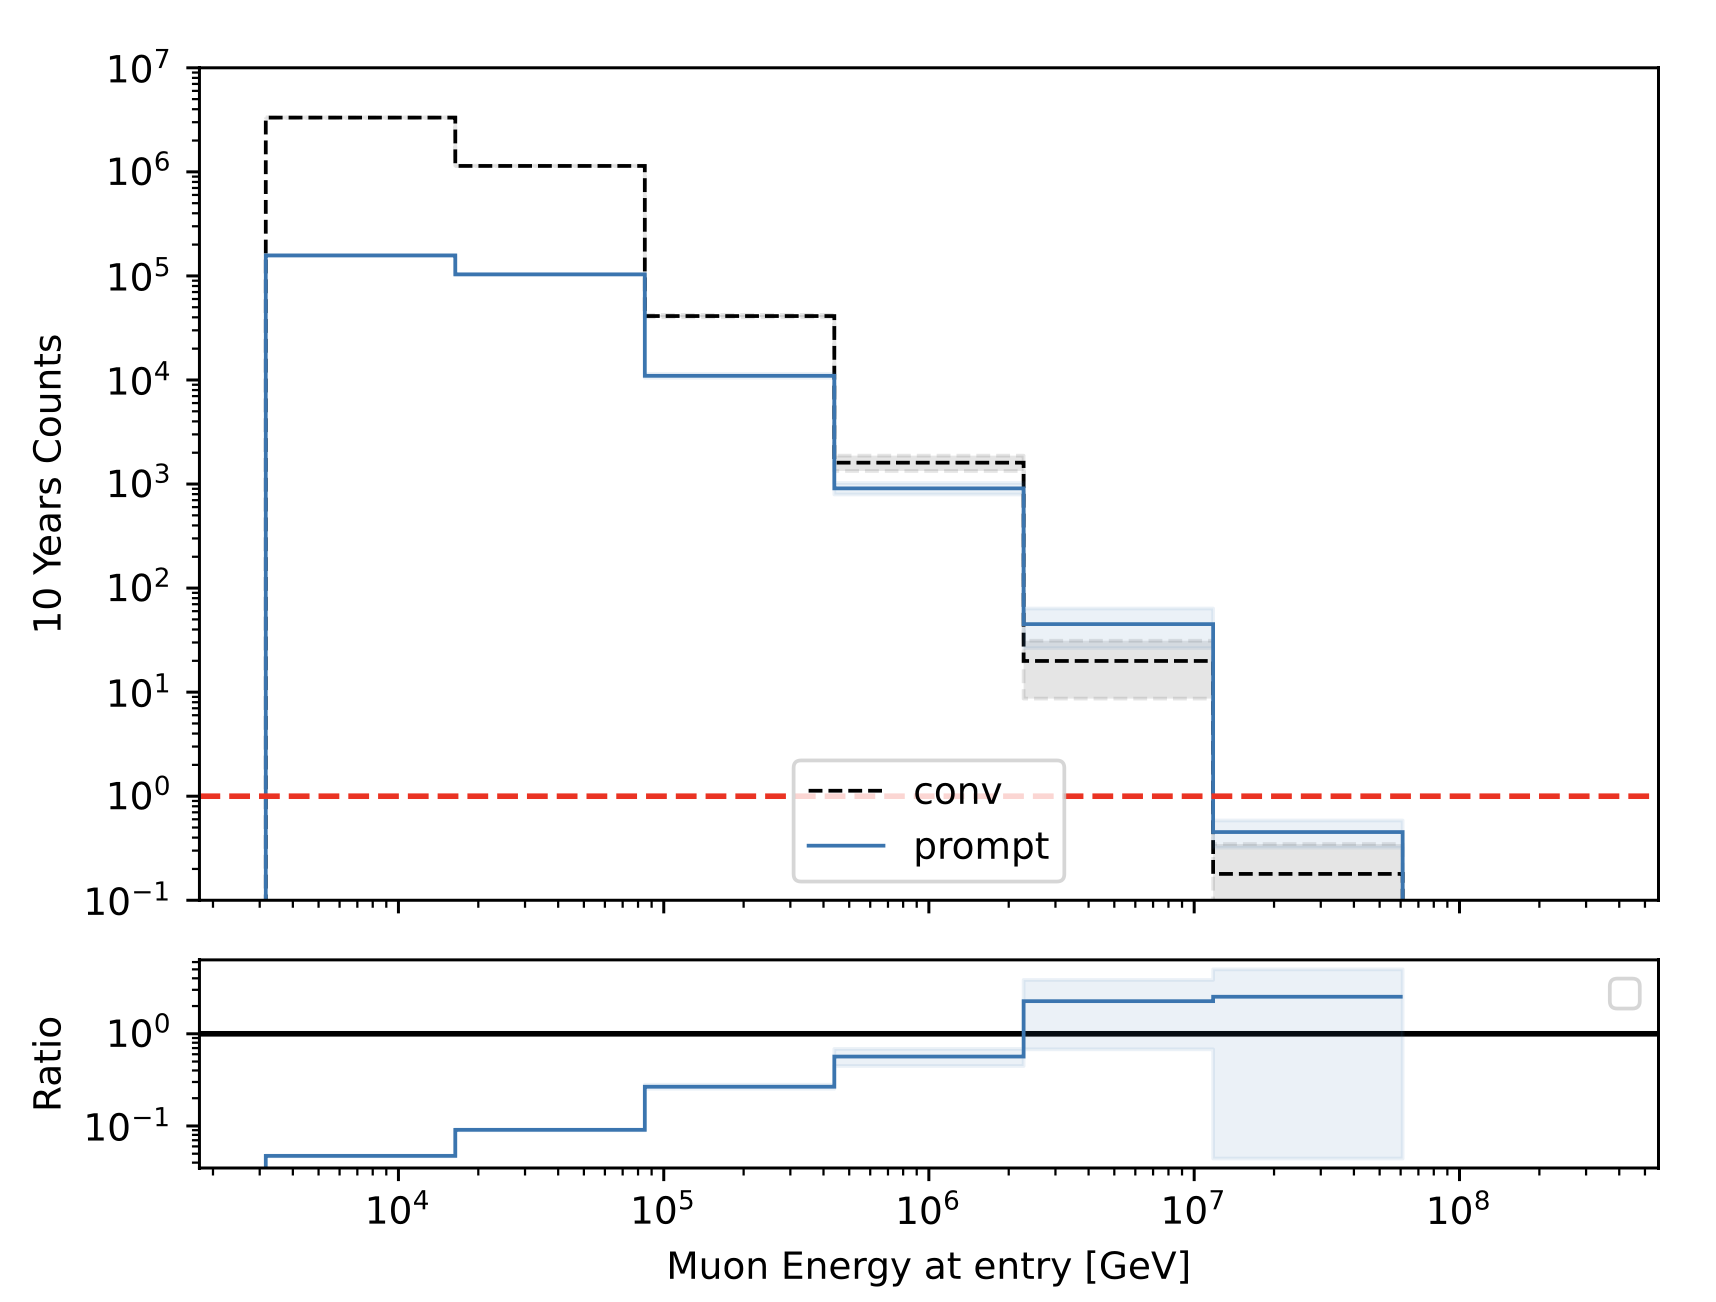
\includegraphics[width=\textwidth]{Plots/spectrum_(3.5,8.5,8)_10Y.png}
    \end{minipage}
    \begin{minipage}{0.39\textwidth}
        \begin{itemize}
            \item Prompt normalization: fraction of prompt component relative to current MC-simulation $n_{pr}$
            \item Poisson likelihood in each histogram bin
            \item Rescale with normalization factors 
            \item Strong model dependency
        \end{itemize}
    \end{minipage}
\end{frame}
\begin{frame}
    \frametitle{Pseudo experiments}
    \begin{minipage}{0.6\textwidth}
        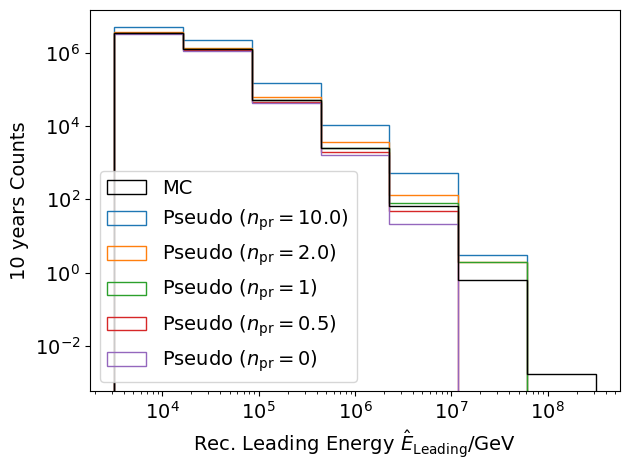
\includegraphics[width=\textwidth]{Plots/injected norms.png}
    \end{minipage}
    \begin{minipage}{0.39\textwidth}
        \begin{itemize}
            \item Testing method based on simulations
            \item Events drawn based on primary model and normalizations
            \item Inject normalization
        \end{itemize}
    \end{minipage}
\end{frame}
\begin{frame}
    \frametitle{Background Estimation}
    \begin{minipage}{0.6\textwidth}
        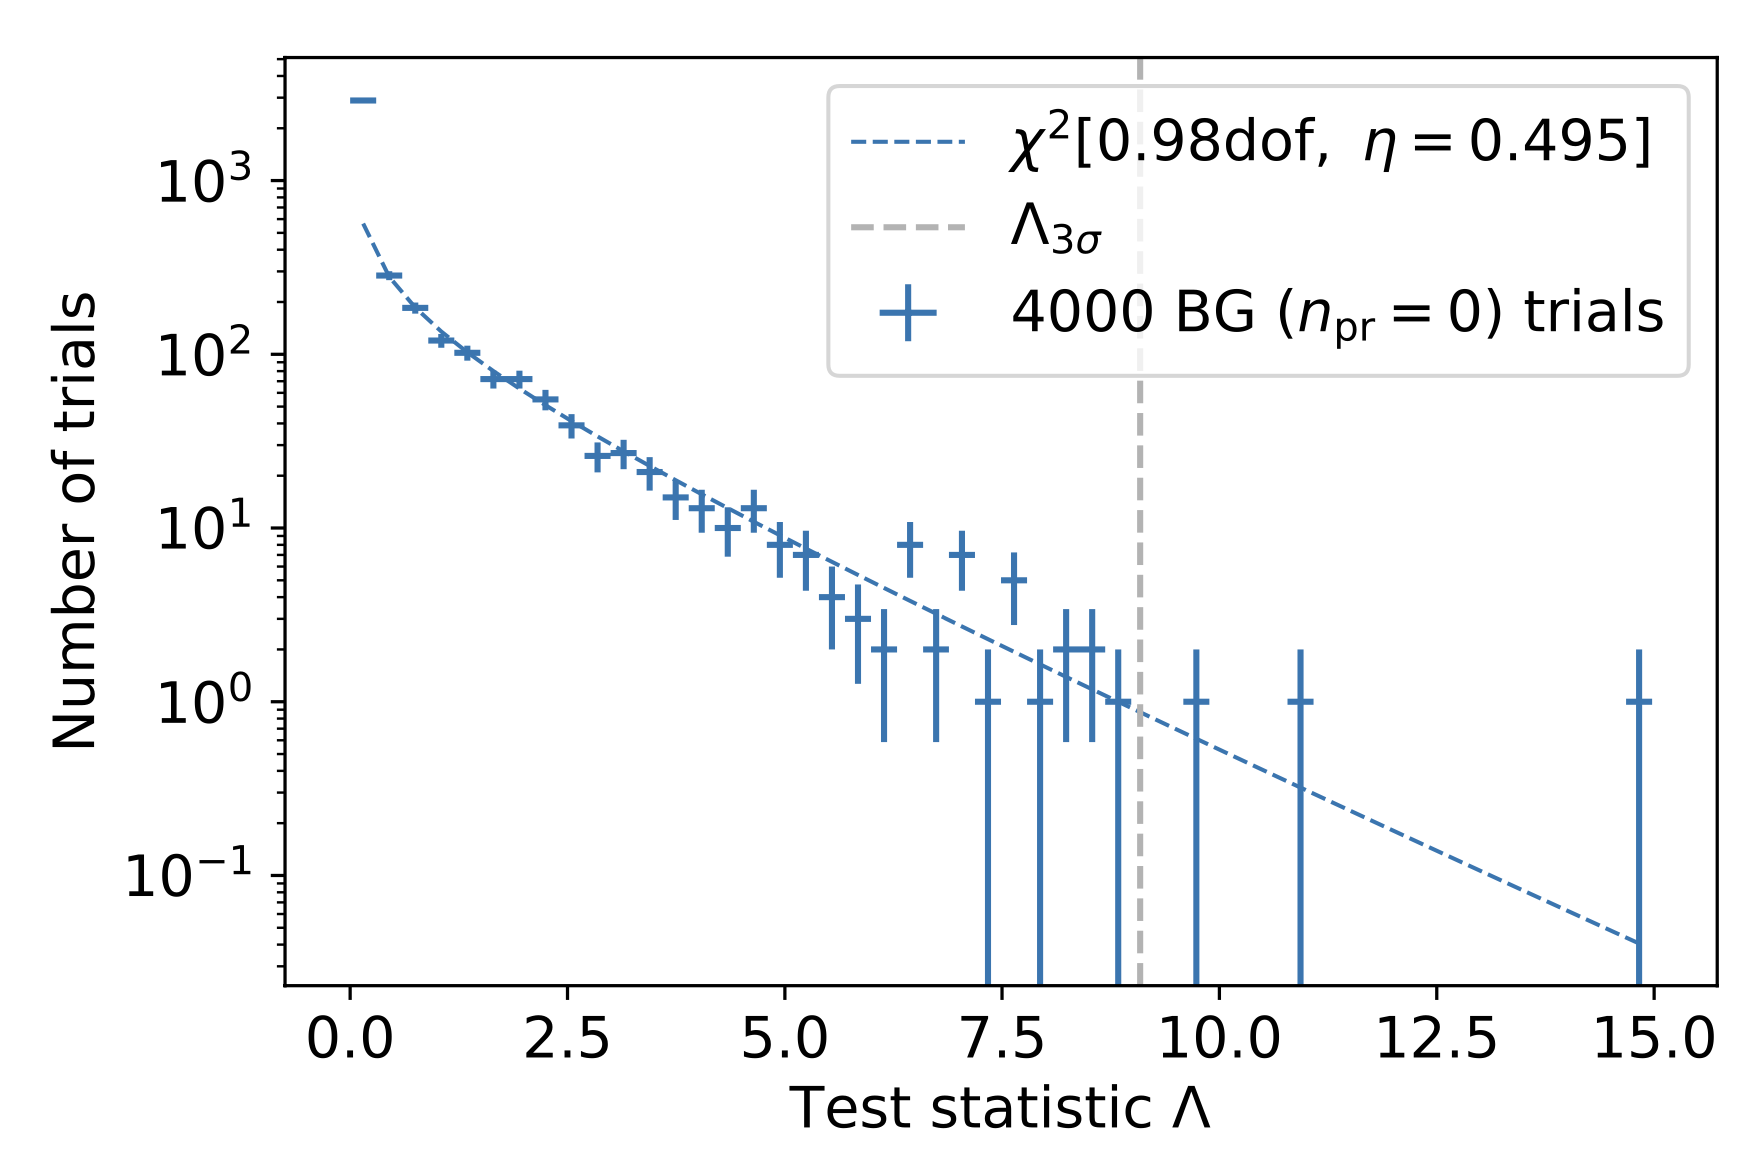
\includegraphics[width=\textwidth]{Plots/background_statistic_chi2_(3.5,8.5,8)_10Yp.png}
    \end{minipage}
    \begin{minipage}{0.39\textwidth}
        \begin{itemize}
            \item Likelihood ratio test
            \item Draw background samples with $n_{pr}=0$
            \item Wilks' theorem: fit $\Chi^2$-distribution
        \end{itemize}
    \end{minipage}
\end{frame}
\begin{frame}
    \frametitle{Discovery Potential: First Estimate}
    \begin{minipage}{0.6\textwidth}
        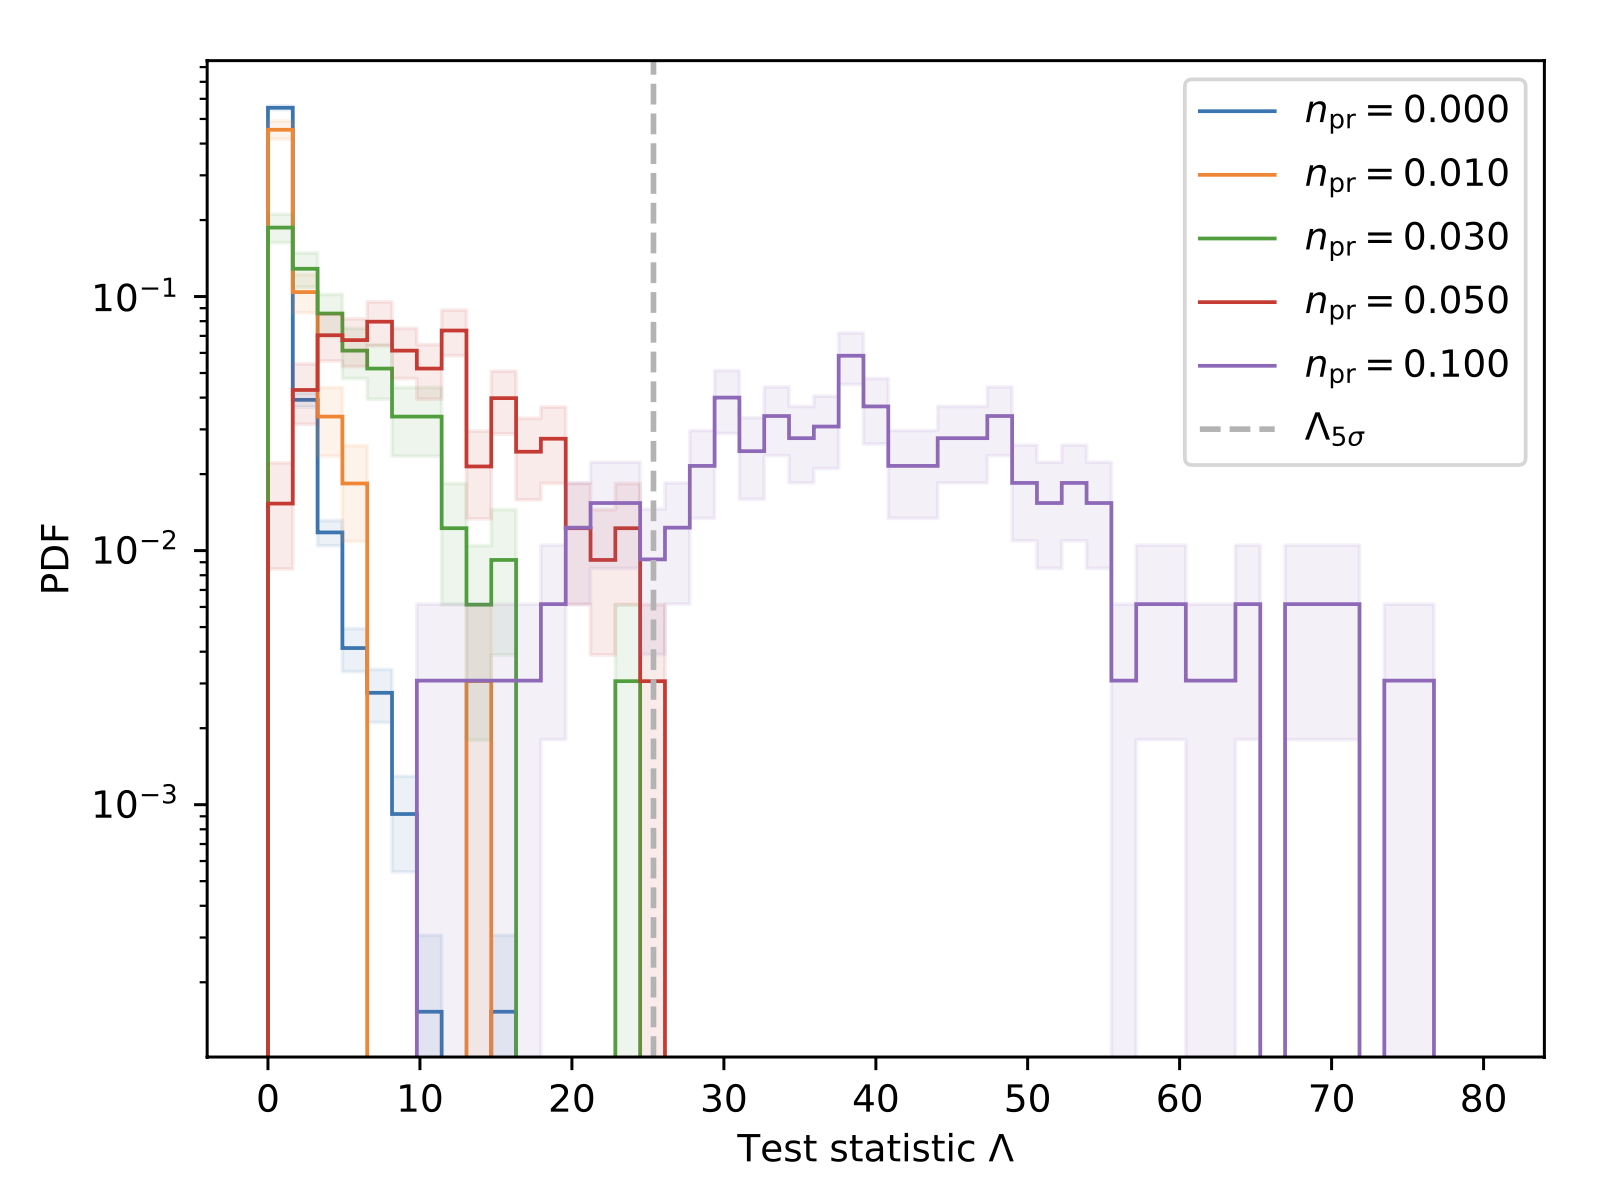
\includegraphics[width=\textwidth]{Plots/TS_Distribution(3.5,8.5,8)_10Y.png}
    \end{minipage}
    \begin{minipage}{0.39\textwidth}
        \begin{itemize}
            \item Prompt norm required to detect it with the current method?
            \item Discovery potential: Norm at which half the generated trials yield $5 \sigma$ significance in the likelihood ratio test
            \item Caution: Systematics are not yet included
	    \item Switch to NNMFit
        \end{itemize}
    \end{minipage}
\end{frame}
\begin{frame}
	\frametitle{Systematic Parameters: SnowStorm}
	\begin{minipage}{0.39\textwidth}
		\begin{itemize}
			\item Detector parameters regarding the ice and DOMs
			\item SnowStorm Ensemble: Individual systematics sampled each event
			\item Drawn from uniform distribution
		\end{itemize}
	\end{minipage}
	\begin{minipage}{0.6\textwidth}
		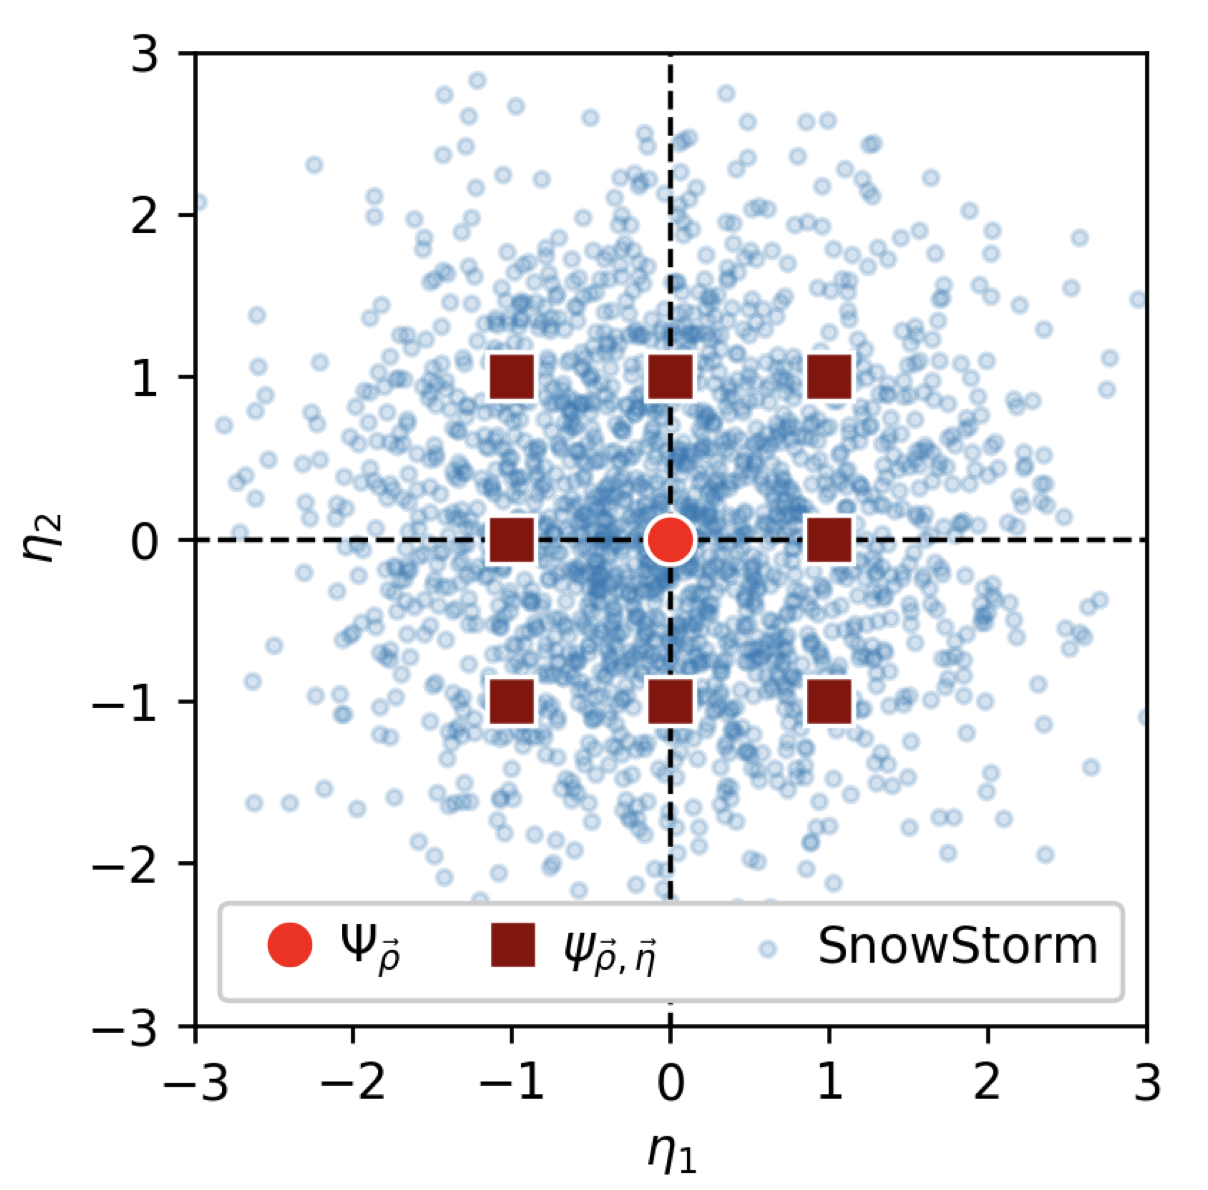
\includegraphics[width=\textwidth]{Plots/SnowStormEnsemble}
	\end{minipage}
\end{frame}
\begin{frame}
	\frametitle{Systematics: Reweighting}
	\begin{minipage}{0.6\textwidth}
		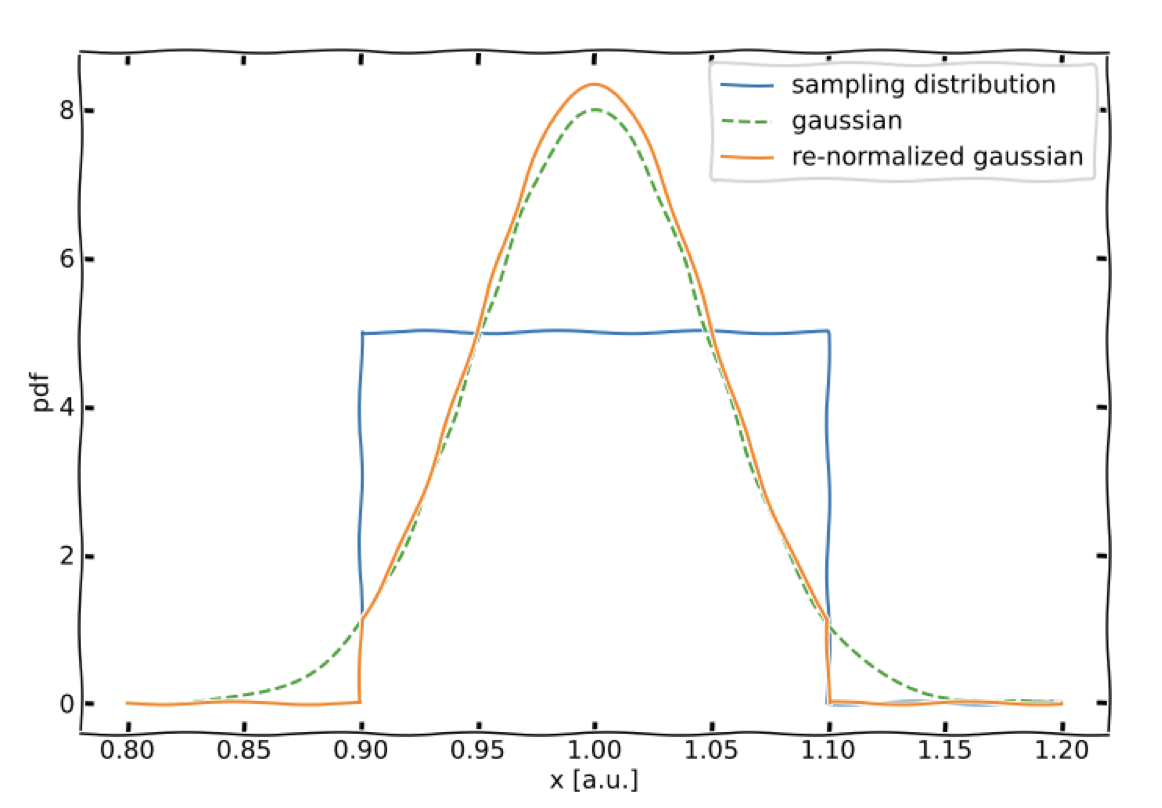
\includegraphics[width=\textwidth]{Plots/SnowStormReweighting}
	\end{minipage}
	\begin{minipage}{0.39\textwidth}
		\begin{itemize}
			\item How do the parameters impact the bincount?
			\item Splitting or reweighting
			\item "Inject" hypothesis for parameter by reweighting
		\end{itemize}
	\end{minipage}
\end{frame}
\begin{frame}
	\frametitle{Detector Parameters}
	\begin{minipage}{0.6\textwidth}
		\includegraphics[width=\textwidth]{Plots/Parameters_impact}
	\end{minipage}
	\begin{minipage}{0.39\textwidth}
		\begin{itemize}
			\item DOM efficiency
			\item Absorption of the ice
			\item Scattering in the ice
			\item Hole-ice models
		\end{itemize}
	\end{minipage}
\end{frame}
\begin{frame}
	\frametitle{Discovery Potential including systematics}
	\begin{figure}
		\centering
		\includegraphics[width=0.49\textwidth]{Plots/asimov_scan_Poisson}
		\includegraphics[width=0.49\textwidth]{Plots/NNMFit_Histogram}
	\end{figure}
\end{frame}
%\begin{frame}
%	\frametitle{What about the MC-uncertainties?}
%	\begin{itemize}
%		\item Good discovery-potential with systematics
%		\item Poisson Likelihood: MC assumed to be perfect estimate
%		\item Alternative: The SAY-likelihood
%	\end{itemize}
%\end{frame}
\begin{frame}
	\frametitle{The SAY-likelihood}
	\begin{itemize}
		\item Poisson likelihood:
        \begin{equation}
            L(k)
	\end{itemize}
\end{frame}
\begin{frame}
	\frametitle{SAY vs Poisson}
	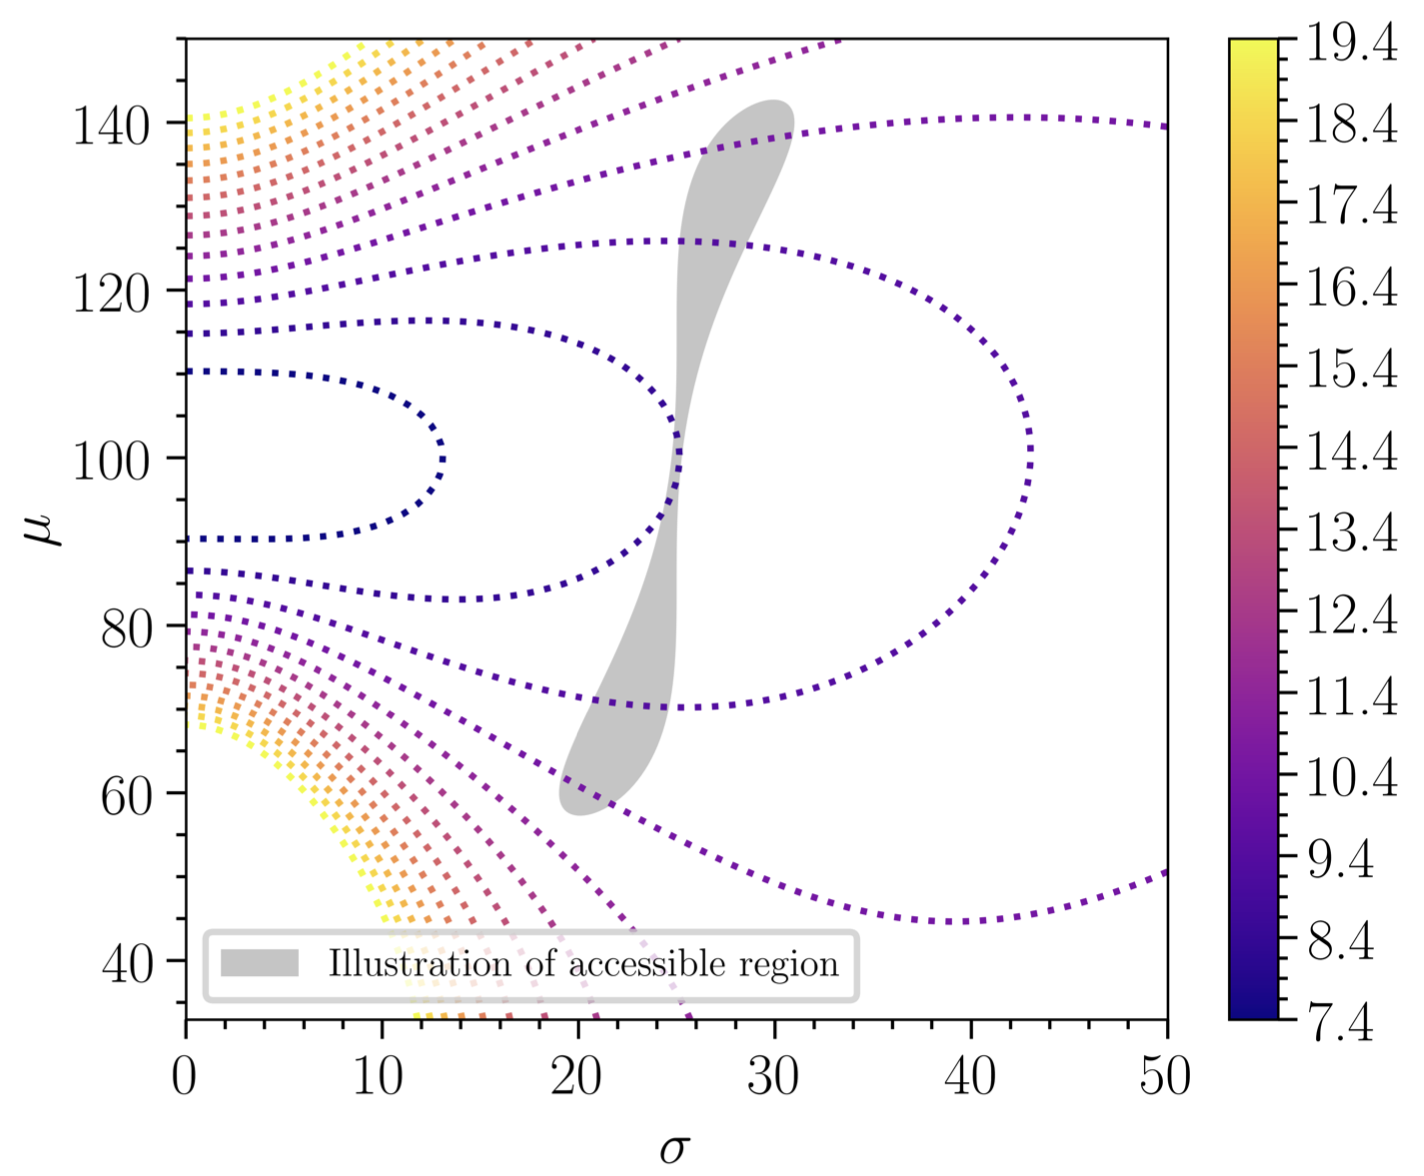
\includegraphics[width=0.8\textwidth]{Plots/SAY_paper}
\end{frame}
\begin{frame}
	\frametitle{Impact of SAY on the fit}
	\begin{figure}
	\end{figure}
\end{frame}
\begin{frame}
	\frametitle{Bias test and fit precision}
	\begin{figure}
		\centering
	\end{figure}
\end{frame}
\begin{frame}
    \frametitle{Summary}
    \begin{minipage}{0.6\textwidth}
        \begin{figure}
            \centering
            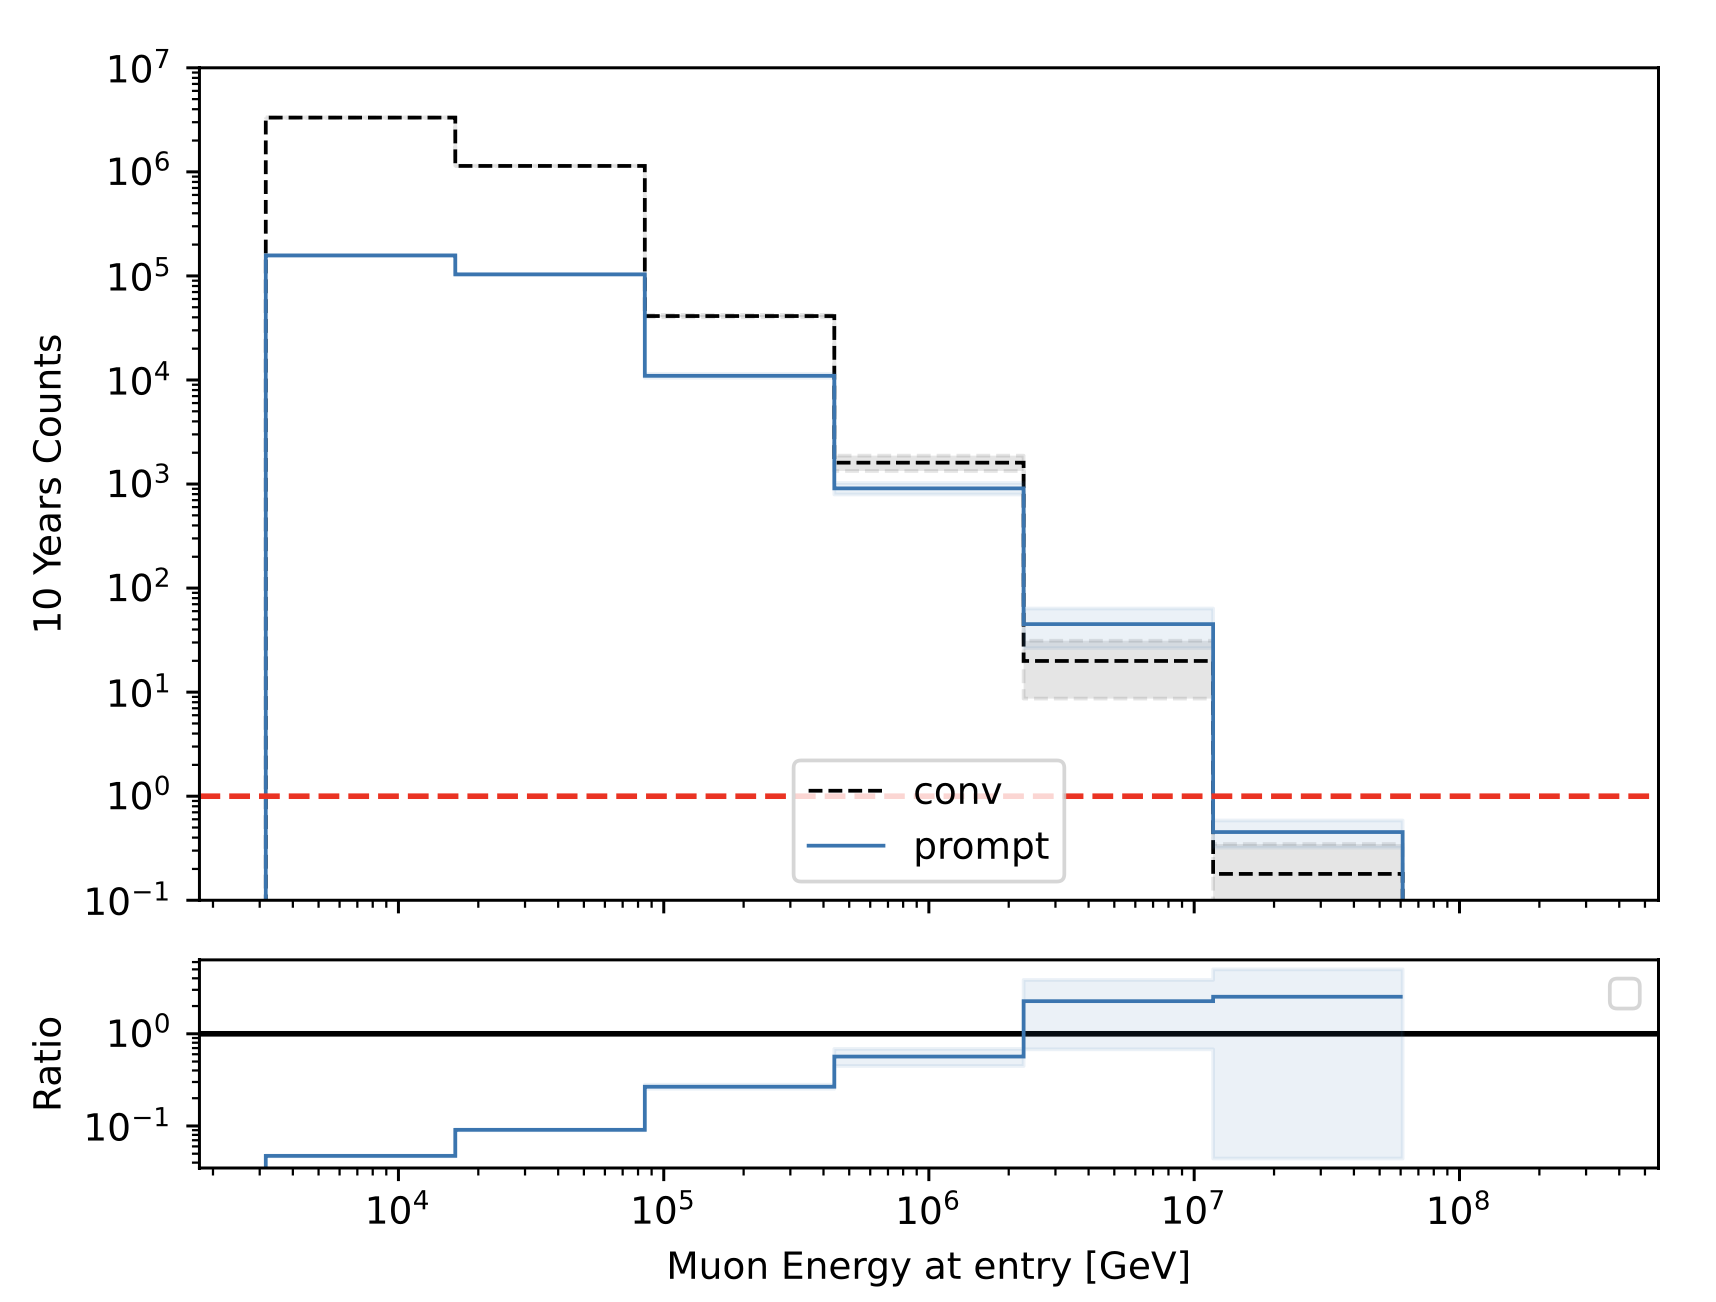
\includegraphics[width=0.5\textwidth]{Plots/spectrum_(3.5,8.5,8)_10Y.png}
            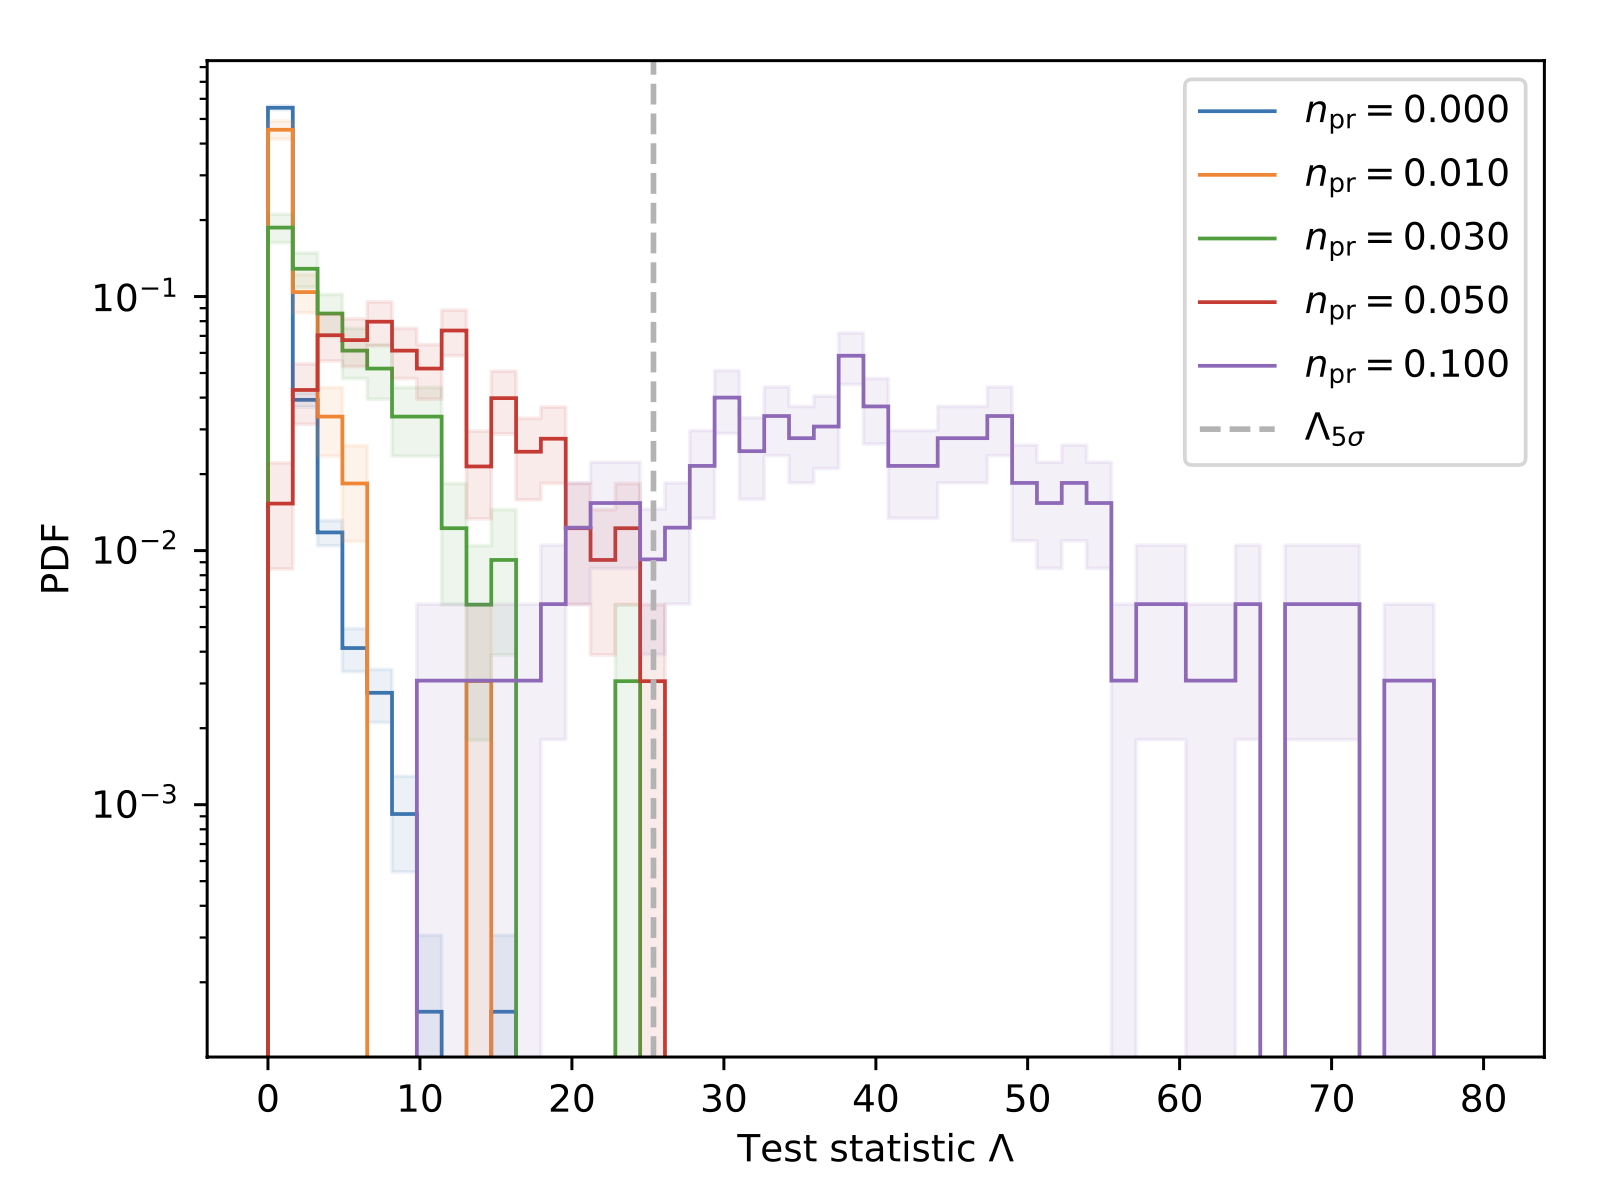
\includegraphics[width=0.5\textwidth]{Plots/TS_Distribution(3.5,8.5,8)_10Y.png}
        \end{figure}
    \end{minipage}
    \begin{minipage}{0.39\textwidth}
        \begin{itemize}
            \item Generate prompt tag in simulation
            \item Simulate up to high energies
            \item Forward fit of prompt normalization
            \item Use MC to estimate significance
        \end{itemize}
    \end{minipage}
\end{frame}
%\begin{frame}
%\end{frame}
\end{document}
